\chapter{Introduction} \label{ch:introduction}
efwefwew
\section{Motivation}
wfwfew
\section{Research Problem}
wfewfe
\section{Objectives}
wefwefw

\section{State of Art}
wfwfewf

\subsection{Quadrotors}
wfwefwe
\subsection{Smartphones as Controllers}
wfwfwewf

\subsection{Smartphone-based Quadrotors}
wfwfwf
\subsection{Quadrotor Flight Modes}
wefwefewfw
\subsubsection{Stabilize Mode}
wfefef
\subsubsection{Altitude Hold Mode}
wefefwefwef
\subsubsection{Loiter Mode}
wfewfefwf
\subsubsection{Return-To-Launch Mode}
wfwefwefw
\subsubsection{Auto Mode}
wfwefwefwe
\section{Outline}
wefwefwefweffew

%\section{Multi-Agent Systems}
%
%
%Advances in exploration and rescue technologies become more relevant than ever before.
%
%In an effort to develop distributed mobile agent systems able to resemble their natural counterparts, engineers have been experimenting with mobile sensor networks trying, for example, to implement flocking applications.  The goal has been to create self-organized networks  capable of coordinated group behaviour \citep{MateiBaras12}. For this purpose, heuristic rules were introduced by \citep{SpanosOlfatiMurray05} in order to explain any form of collective behaviour of a large number of individuals  with a common goal. These rules are known as cohesion, separation, and alignment. Cohesion means the attempt to stay close to  the neighbours, separation means avoiding collisions with neighbours, and alignment means the attempt to match velocity with neighbour agents. 
%
%
% For example, oil spilled in the sea generates a scalar field of oil concentration values (Fig. \ref{fig:oilspill}). Similarly,  radiation levels after  nuclear disaster like in Fukushima (Fig.  \ref{fig:fukushima_1}), or a toxic substance cloud moving in space are  phenomena that can be represented as scalar fields (Fig. \ref{fig:scalarfieldsource}). 
%\afterpage{
%\begin{figure}[ht!]
%        \centering
%        \begin{subfigure}[t]{0.49\textwidth}
%                \includegraphics[width=\textwidth]{oilspill.eps}
%                \caption{Oil spill \footnotemark} 
%                \label{fig:oilspill}
%        \end{subfigure}%
%        ~ %add desired spacing between images, e. g. ~, \quad, \qquad etc.
%          %(or a blank line to force the subfigure onto a new line)
%        \begin{subfigure}[t]{0.49\textwidth}
%                \includegraphics[width=\textwidth]{fukushima_1.eps}
%                \caption{Fukushima's environment radiation levels after nuclear disaster  \footnotemark}
%                \label{fig:fukushima_1}
%        \end{subfigure}
%        ~ %add desired spacing between images, e. g. ~, \quad, \qquad etc.
%          %(or a blank line to force the subfigure onto a new line)
%        \begin{subfigure}[t]{0.62\textwidth}
%                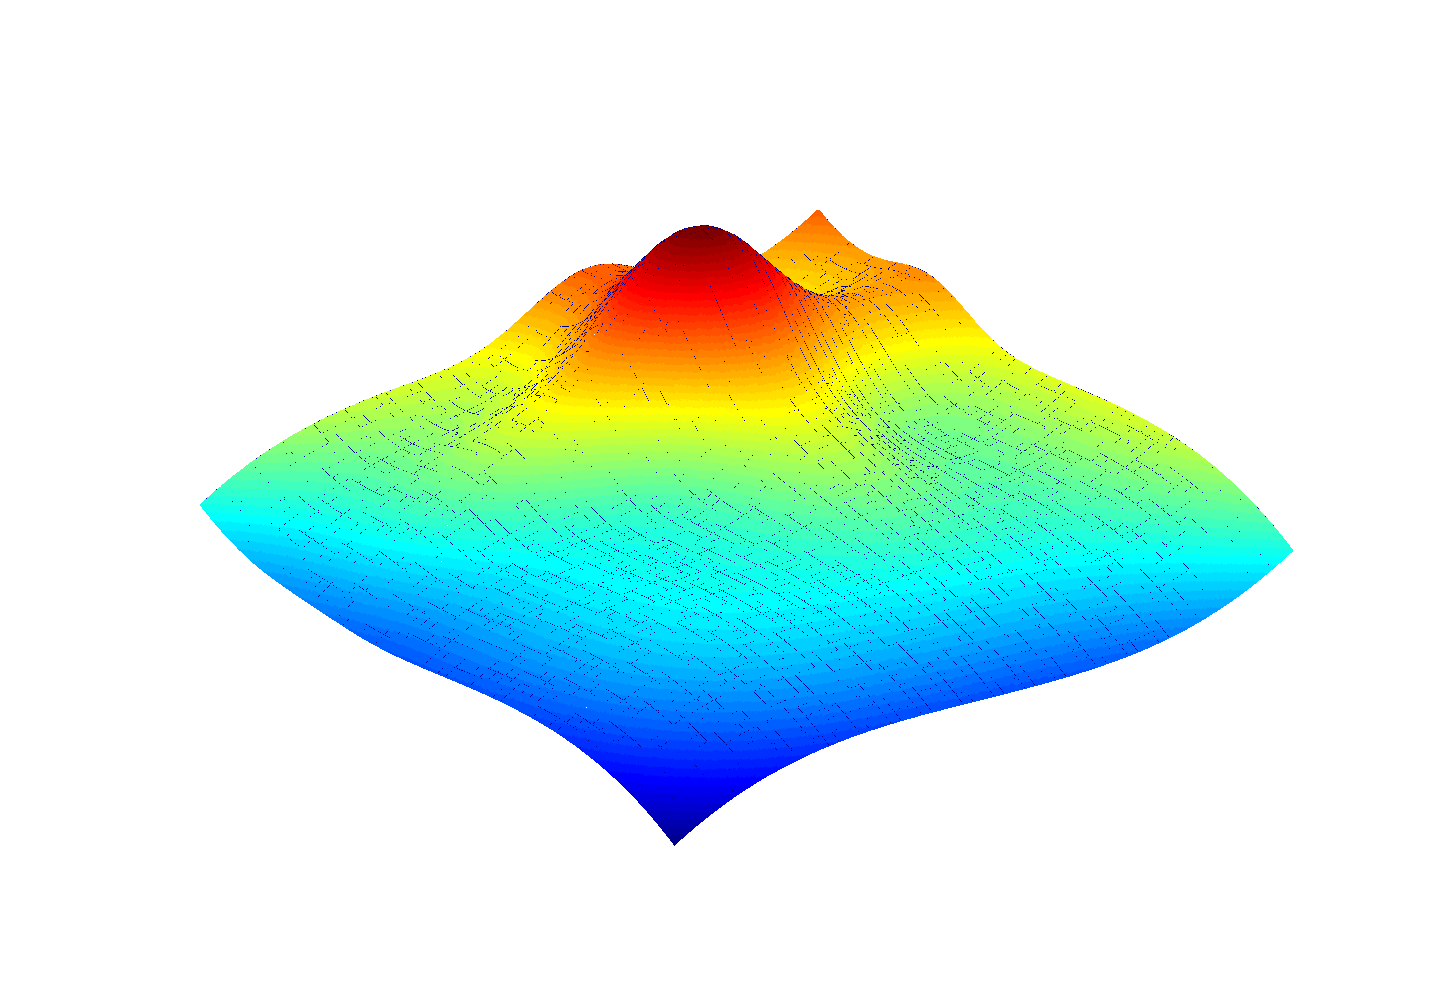
\includegraphics[width=\textwidth]{scalarfieldsource.eps}
%                \caption{Toxic cloud}
%                \label{fig:scalarfieldsource}
%        \end{subfigure}%
%        ~ %add desired spacing between images, e. g. ~, \quad, \qquad etc.
%          %(or a blank line to force the subfigure onto a new line)
%       \caption{Scalar fields} \label{fig:scalar field}
%\end{figure}
%\footnotetext[1]{Picture taken from FeedNetBack project}
%\footnotetext[2]{Picture taken from seaandskyjp.wordpress.com}
%}
% 


